\chapter{Fundamentos}
\label{cha:foundation}

Neste capítulo serão discutidos alguns conceitos básicos utilizados como fundação no desenvolvimento da solução assim como alguns detalhes técnicos relacionados a linguagem de programação Go necessários para o entendimento dos mecanismos implementados em Rivers e discutidos em capítulos seguintes.

\section{Streams}
\label{sec:streams}

Streams são definidos como uma sequência de dados que são produzidos assincronamente ao longo do tempo fluindo de sua fonte conhecida como upstream à um destino chamado de downstream \cite{article:tim:streams}. Frequentemente streams são comparados à coleções de dados como por exemplo arrays e listas. No entanto streams diferentemente de coleções não definem necessariamente um tamanho fixo, podendo produzir elementos indefinidamente ao longo do ciclo de vida de um programa. Apesar desta diferença, as APIs de streams são muitas vezes modeladas de maneira que se assemelham a APIs de manipulação de coleções compartilhando muitas das operações como \emph{filter}, \emph{map}, \emph{reduce} etc.

Streams são amplamente aplicados no âmbito computacional no entanto em muitos casos seus conceitos não são explicitamente aparentes. Um exemplo clássico são os \emph{Unix Pipes}, mecanismos utilizados para realizar comunicação entre processos \cite{book:tanenbaum:ipc} via canais de comunicação conhecidos como standard input e output ou simplesmente \emph{stdin} e \emph{stdout} respectivamente. Uma operação de pipe conecta o canal stdout de um programa ao stdin de outro permitindo com que dados sejam transmitidos de um lado ao outro passando por diferentes estágios de processamento específicos a cada programa. A figura \ref{fig:unix_pipes} mostra os comandos Unix \emph{find}, \emph{grep} e \emph{wc} sendo combinados via operações de \emph{pipe} formando um pipeline com três estágios de processamento.

As aplicações de streams são tantas que muitas linguagens de programação adotam completamente os seus conceitos e disponibilizam APIs robustas que permitem a criação de pipelines complexos de processamento de stream de dados, alguns exemplos são \cite{docs:nodejs:streams}, \cite{docs:haskell:streams} e \cite{docs:java8:streams}.

\begin{figure}[H]
  \includegraphics[width=0.55\textwidth]{unix-pipes}
  \centering
  \caption{Exemplo de stream pipeline em Unix.}
  \label{fig:unix_pipes}
\end{figure}

\section{Golang}
\label{sec:golang}

Go é uma linguagem de programação open source, estaticamente tipada \cite{paper:microsoft:static_typing} com suporte a garbage collector \cite{paper:sun:gc} criada pela Google com foco em simplicidade, produtividade e concorrência. O sistema de tipos da linguagem aborda de maneira inovadora alguns conceitos como por exemplo interfaces \cite{article:wikipedia:interfaces} que difere do conceito tradicional implementado por linguagens como Java. Outro aspecto interessante da linguagem é seu modelo de concorrência baseado em Goroutines \cite{docs:golang:goroutine} conceito similar ao de Coroutines \cite{article:wikipedia:coroutines} e troca de mensagens \cite{lecture:ucl:message_passing} através do uso de canais de comunicação. A seguir serão apresentados alguns dos conceitos da linguagem que foram essenciais na implementação de Rivers.

\subsection{Interfaces}
\label{subsec:interfaces}

Interface é o mecanismo através do qual sistemas podem ser modelados visando reuso e extensibilidade. Contratos abstratos são especificados descrevendo determinadas funcionalidades de um sistema independente de possíveis implementações, isso permite com que qualquer componente satisfazendo uma determinada interface possa ser utilizado como provedor da funcionalidade em questão. Em muitas linguagens de programação como Java, componentes precisam explicitamente declarar sua intenção de implementar uma interface e com isso sendo necessário definir as interfaces necessárias de um sistema como parte da modelagem da solução e consequentemente tornando a solução menos suscetível a futuras alterações de design. O código \ref{code:java:interfaces} mostra um exemplo de uma classe Java implementando uma interface específica.

\begin{figure}[H]
  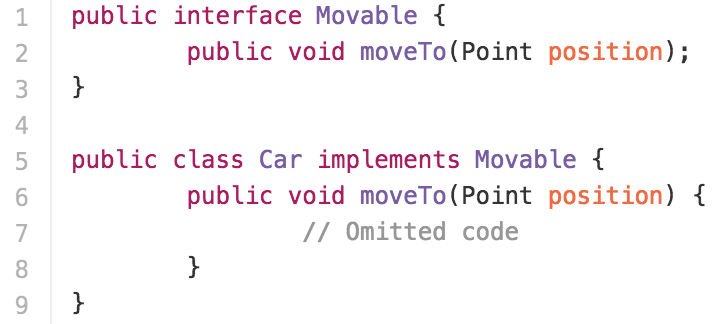
\includegraphics[width=0.65\textwidth]{java_interfaces}
  \centering
  \caption{Exemplo de implementação de uma interface em Java.}
  \label{code:java:interfaces}
\end{figure}

Em Go, interfaces são satisfeitas implicitamente sem a necessidade de que componentes declararem explicitamente sua intenção de implementar uma interface eliminando assim hierarquias de dependências presentes em linguagens orientadas à objetos \cite{book:learn_oop}. Para que um componente A satisfaça a interface B, A deve simplesmente implementar todos os métodos declarados em B. Desta maneira decisões arquiteturais de sistema podem ser tomadas em momentos futuros a medida em que novos casos de uso são introduzidos e padrões de código detectados evoluindo assim a arquitetura gradativamente. O código a seguir mostra como o exemplo Java em \ref{code:java:interfaces} pode ser reescrito em Go. Note que o tipo Car não possui qualquer dependência com a interface Movable ao contrário da versão Java, porém pode ser utilizado como um tipo Movable por implementar o método MoveTo na linha 7.

\begin{figure}[H]
  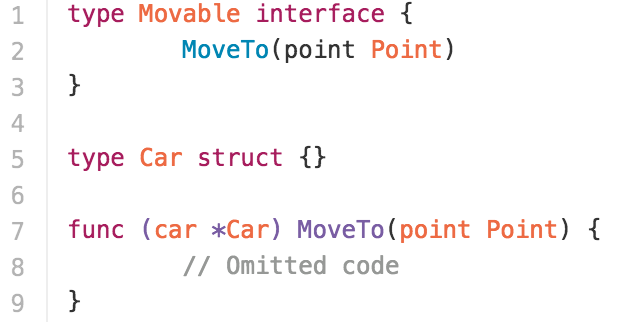
\includegraphics[width=0.5\textwidth]{go_interfaces}
  \centering
  \caption{Exemplo de implementação de uma interface em Go.}
  \label{code:go:interfaces}
\end{figure}

Em \ref{sec:rivers:architecture} será discutido como Rivers faz o uso de interfaces para definir os building blocks do framework permitindo novas funcionalidades sejam introduzidas à arquitetura de maneira transparente e não intrusiva.

\begin{flushright}
\mbox{}\vfill
{\sffamily\itshape
``Note too that the elimination of the type hierarchy also eliminates a form of dependency hierarchy. Interface satisfaction allows the program to grow organically without predetermined contracts. And it is a linear form of growth; a change to an interface affects only the immediate clients of that interface; there is no subtree to update. The lack of implements declarations disturbs some people but it enables programs to grow naturally, gracefully, and safely.
''\\}
--- \textsc{Rob Pike}
\end{flushright}

\subsection{Goroutines}
\label{subsec:goroutines}

Goroutine é o mecanismo que a linguagem Go utiliza para executar código de maneira concorrente e potencialmente em paralelo de maneira similar a outros mecanismos como por exemplo \cite{article:wikipedia:coroutines} e \cite{article:wikipedia:threads} porém com algumas diferenças que faz com que seu papel no modelo de concorrência da linguagem seja crucial. Goroutines são basicamente funções que executam assincronamente e concorrentemente utilizando o comando go e são gerenciadas pelo runtime da linguagem. Ao contrário de threads que exigem pelo menos 1MB de memória inicial para inicialização, Goroutines são extremamente baratas sendo necessário apenas 2KB de memória para inicialização podendo ajustar este valor sob demanda alocando e desalocando espaço na Heap, permitindo com que centenas de milhares de Goroutines possam ser executadas concorrentemente. Além disso o custo de troca de contexto entre Goroutines é extremamente baixo comparado com threads uma vez que Goroutines são genrenciadas pelo runtime e ao contrário de threads não necessitam acessar recursos do Sistema Operacional para realizar a troca de contexto. \cite{blog:how_goroutines_work} faz uma excelente análise do funcionamento de Goroutines em comparação com o funcionamento de OS threads. A figura \ref{code:goroutine:example} mostra uma Goroutine sendo criada na linha 16 utilizando o comando go para executar assincronamente a função say com o parâmetro "world".

\begin{figure}[H]
  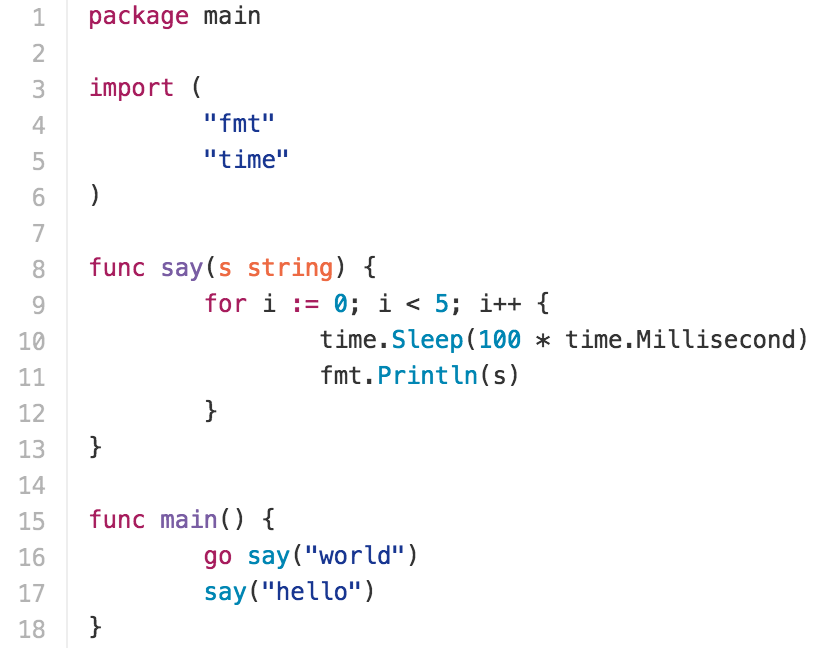
\includegraphics[width=0.75\textwidth]{goroutine_example}
  \centering
  \caption{Exemplo de uso de Goroutines.}
  \label{code:goroutine:example}
\end{figure}

\subsection{Channels}
\label{subsec:channels}

Channel é o mecanismo básico utilizado para realizar a comunicação entre Goroutines via troca de mensagem e a sincronização de suas execuções permitindo que dados sejam enviados de uma Goroutine à outra de maneira segura sem a necessidade de compartilhar memória e é a base para o modelo Produtor-Consumidor \cite{paper:david_kocher:producer_consumer} utilizado como fundação na implementação de Rivers.

Dados são escritos e lidos de um Channel de maneira síncrona sendo desnecessário o uso de outras primitivas de concorrência como por exemplo semáforos ou mutex \cite{paper:concurrency:schmidt}. Por padrão uma Goroutine ao escrever um dado em um Channel bloqueia sua execução até que outra Goroutine leia este dado do Channel liberando espaço para que outro dado seja escrito. No entanto um Channel pode ser criado com um Buffer permitindo com que vários dados possam ser escritos no Channel sem que sejam consumidos, bloqueando então apenas quando não houver mais espaço no Buffer. Channels podem ser de somente escrita, somente leitura ou ambos permitindo implementar alguns padrões de design interessantes como por exemplo Pipeline Pattern \cite{docs:golang:pipeline_pattern}. A figura a seguir mostra um exemplo de criação de um Channel com um Buffer de capacidade 2 na linha 2 e duas mensagens enviadas no canal nas linhas 3 e 4 e logo em seguida consumidas nas linhas 6 e 7. 

\begin{figure}[H]
  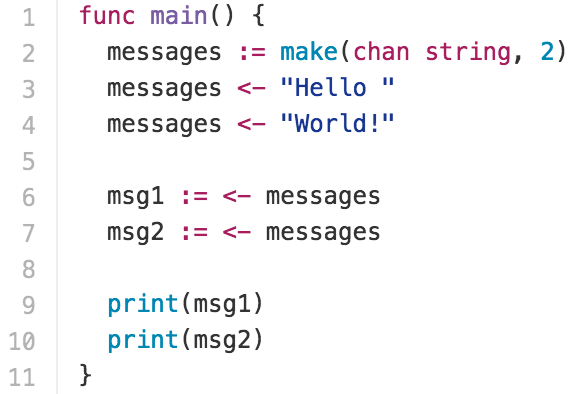
\includegraphics[width=0.55\textwidth]{channels_example}
  \centering
  \caption{Exemplo de uso de Channels.}
  \label{code:channels:example}
\end{figure}
